%% This file is generated by Jinja2
% Template for drawing GPS figure
% Author: Long Gong
\documentclass[border=2pt]{standalone}
%%%<
\usepackage{verbatim}
%%%>
\begin{comment}
:Title: Template for GPS Figure
:Author: Long Gong

A template for GPS figure. 

In some ways, this TeX script works as the "model" of our application 
for visualizing a GPS simulation results. 

Parameters:
    width: scalar, total length of x axis
    height: scalar, total length of y axis
    xlabels: list, labels for x axis
    ylabels: list, labels for y axis
    flows: list of dict, packets in each flow, its detailed structures 
           look like as follows,
            [{
               "id": <flow id>,
               "packets": [
               {
                "v_start_time": <virtual start time>,
                "v_finish_time": <virtual finish time>,
                "y_min": <bottom border value>,
                "y_max": <top border value>
               },
               ...
               ] 
            },
            ...
            ]

Programmed in TikZ by Long Gong. Templating language is Jinja2, 
templaing syntax is the default setting of Jinja2.
\end{comment}

\usepackage{tikz}
\usetikzlibrary{shapes, positioning}



\begin{comment}
%% detailed results %%
#flow id, virtual start time, virtual finish time, real start time, real finish time
1, 0, 2.0, 0, 4.0
1, 2.0, 5.0, 1, 13.0
1, 5.0, 11.0, 2, 28.0
2, 0.0, 6.0, 0, 16.0
2, 6.0, 9.0, 1, 25.0
3, 0.0, 3.0, 0, 7.0
3, 3.0, 4.0, 1, 10.0
3, 4.0, 10.0, 2, 27.0

\end{comment}

\begin{document}
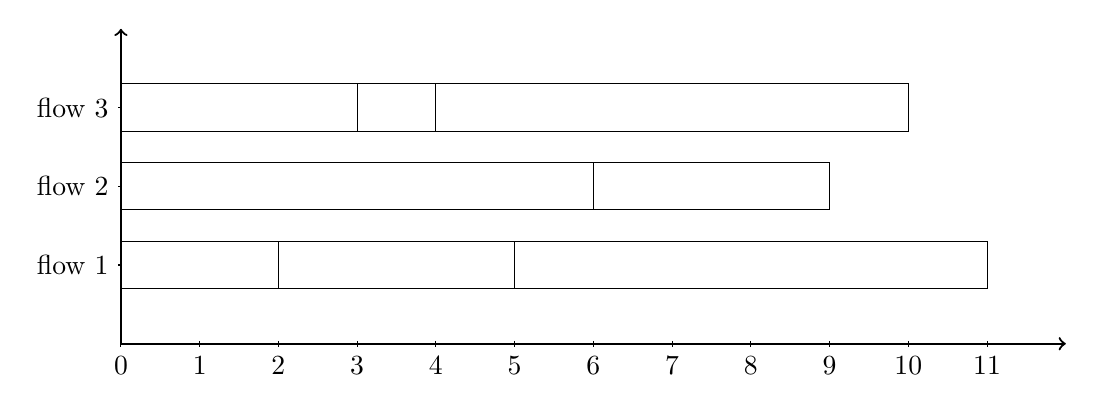
\begin{tikzpicture}


%% place x axis label
    \draw (0, 1pt) -- (0, -1pt) node[anchor=north] {$0$};
    \draw (1, 1pt) -- (1, -1pt) node[anchor=north] {$1$};
    \draw (2, 1pt) -- (2, -1pt) node[anchor=north] {$2$};
    \draw (3, 1pt) -- (3, -1pt) node[anchor=north] {$3$};
    \draw (4, 1pt) -- (4, -1pt) node[anchor=north] {$4$};
    \draw (5, 1pt) -- (5, -1pt) node[anchor=north] {$5$};
    \draw (6, 1pt) -- (6, -1pt) node[anchor=north] {$6$};
    \draw (7, 1pt) -- (7, -1pt) node[anchor=north] {$7$};
    \draw (8, 1pt) -- (8, -1pt) node[anchor=north] {$8$};
    \draw (9, 1pt) -- (9, -1pt) node[anchor=north] {$9$};
    \draw (10, 1pt) -- (10, -1pt) node[anchor=north] {$10$};
    \draw (11, 1pt) -- (11, -1pt) node[anchor=north] {$11$};

%% place y axis label
    \draw (1pt, 1) -- (-1pt, 1) node[anchor=east] {flow $1$};
    \draw (1pt, 2) -- (-1pt, 2) node[anchor=east] {flow $2$};
    \draw (1pt, 3) -- (-1pt, 3) node[anchor=east] {flow $3$};

% flows
% flow 1
\filldraw[fill=white, draw=black] (0, 0.7 ) rectangle (2.0, 1.3);
\filldraw[fill=white, draw=black] (2.0, 0.7 ) rectangle (5.0, 1.3);
\filldraw[fill=white, draw=black] (5.0, 0.7 ) rectangle (11.0, 1.3);
% flow 2
\filldraw[fill=white, draw=black] (0.0, 1.7 ) rectangle (6.0, 2.3);
\filldraw[fill=white, draw=black] (6.0, 1.7 ) rectangle (9.0, 2.3);
% flow 3
\filldraw[fill=white, draw=black] (0.0, 2.7 ) rectangle (3.0, 3.3);
\filldraw[fill=white, draw=black] (3.0, 2.7 ) rectangle (4.0, 3.3);
\filldraw[fill=white, draw=black] (4.0, 2.7 ) rectangle (10.0, 3.3);

%% virtual time axis (remove labels)
% node[anchor=north west] {}
%  node[anchor=south east] {}
\draw[thick,->] (0,0) -- (12,0) ;
\draw[thick,->] (0,0) -- (0,4);

\end{tikzpicture}
\end{document}